\documentclass[twoside,a4paper]{report}
\usepackage[italian]{babel}
\usepackage[utf8]{inputenc}
\usepackage{amsmath}
\usepackage{amsthm}
\usepackage{amsfonts}
\usepackage{amssymb}
\usepackage{cancel}
\usepackage[margin=1in]{geometry}
\usepackage{hyperref}
\usepackage{bookmark}
\usepackage{setspace}
\usepackage{titlesec}
\usepackage{fancyhdr}
\usepackage{adjustbox}
\usepackage{float}
\usepackage{graphicx}

\graphicspath{{./images/}}

\setlength{\parskip}{0pt}
\titlespacing*{\subparagraph}{1em}{0em}{0em} 

\makeatletter
\renewenvironment{abstract}{%
    \if@twocolumn
        \section*{\abstractname}%
    \else
        \begin{center}%
            {\bfseries \abstractname\vspace{-.5em}\vspace{\z@}}%
        \end{center}%
        \small
        \begin{quotation}
    \fi}
    {\if@twocolumn\else\end{quotation}\fi}
\makeatother

\hypersetup{
    pdfauthor={Luca Facchini},
    pdftitle={Appunti di Sistemi Informativi},
    pdfsubject={Appunti del corso di Sistemi Informativi, tenuto dal prof. Bouquet Paolo presso l'Università degli Studi di Trento. Corso seguito nell'anno accademico 2024/2025.},
    pdfkeywords={Sistemi Informativi, Università degli Studi di Trento, Paolo Bouquet},
    pdfproducer={LaTeX},
    pdfcreator={pdflatex},
}

\fancypagestyle{chapterInit}{%
    \fancyhf{}
    \renewcommand{\headrulewidth}{0pt}
    \fancyfoot{}
    \fancyfoot[LE,RO]{\thepage}
    \fancyfoot[LO,RE]{"Appunti di Sistemi Informativi" di Luca Facchini}
}
\fancypagestyle{stdPage}{
    \fancyhead{}
    \fancyhead[LE]{\leftmark}
    \fancyhead[RO]{\rightmark}
    \setlength{\headheight}{15pt}
    \fancyfoot{}
    \fancyfoot[LE,RO]{\thepage}
    \fancyfoot[LO,RE]{"Appunti di Sistemi Informativi" di Luca Facchini}
    \renewcommand{\footrulewidth}{0.4pt}
}

\newtheorem{definition}{Definizione}[chapter]


\title{Appunti di Sistemi Informativi}
\author{Luca Facchini (mat. 245965)}
\date{A.A. 2024/2025}

\begin{document}
    \begin{titlepage}
        \centering  % Center everything on the title page
        {\Huge\textbf{Appunti di Sistemi Informativi}} \\[1cm] % Title
        \vspace{0.5cm}
        
        {\Large Luca Facchini} \\ % Author name
        \vspace{0.3cm}
        {\large Matricola: 245965} \\[2cm] % Additional author info
        
        {\large Corso tenuto dal prof. Casari Paolo} \\[0.3cm] % Course information
        {\large Università degli Studi di Trento} \\[1.5cm]
        
        {\large A.A. 2024/2025} \\[3cm] % Academic year
        
        % Abstract section with spacing control
        \vfill
        \begin{abstract}
            Questo documento contiene gli appunti del corso di Sistemi Informativi, tenuto dal prof. Casari Paolo presso l'Università degli Studi di Trento. Il corso è stato seguito nell'anno accademico 2024/2025.\footnote{Dove non specificato diversamente eventuali immagini provengono dalle slide del corso (o da materiale didattico fornito dal docente) le quali sono fornite e tratte dal libro: "Sistemi Informativi Aziendali" di Pighin M. e Mazona A. solo per le immagini possono essere soggette a copyright e comunque usabili solo per fini didattici e in base alla legge italiana sul diritto d'autore (al massimo 15\%).}
        \end{abstract}
        
        \vfill  % Pushes the content to the center vertically
    \end{titlepage}

    \pagestyle{stdPage}
    
    \addtocontents{toc}{\protect\thispagestyle{stdPage}}
    \begingroup
        \tableofcontents
        \thispagestyle{stdPage}
    \endgroup
    
    \include{chapters/01-laSocietàDellaConoscenza}
    \chapter{Concetti Generali sull'Informatica Aziendale}
\thispagestyle{chapterInit}
\section{Introduzione e definizioni}
    \paragraph{Informatica Aziendale} L'\textbf{informatica aziendale} è la disciplina che studia l'applicazione dell'informatica nelle aziende, studia inoltre l'influenza di questa nelle diverse categorie di un sistema aziendale. Esistono diversi settori di applicazione trai quali:
        \begin{itemize}
            \item \textbf{Aiuto e guida operativa} - Assistenza agli operatori a seguire le corrette procedure di lavoro con un costante controllo iterativo sui dati. Facilitazione di ricerca e recupero di informazioni.
            \item \textbf{Organizzativa} - Automazione di processi da un lato, richiesta di \textbf{competenze} e \textbf{risorse} differenti dall'altro.
            \item \textbf{Controllo} - Rilevazione di caratteristiche e comportamenti di un sistema, possibilità di \textbf{analisi quantitative} e \textbf{qualitative}.
            \item \textbf{Strategia} - Supporto ai processi di trasformazione e innovazione, supporto alle decisioni strategiche. 
        \end{itemize}
    \paragraph{Sistemi Informativi aziendali} I \textbf{sistemi informativi aziendali} sono l'insieme delle procedure e delle infrastrutture che definiscono e supportano l'elaborazione, la distribuzione e l'utilizzo delle informazioni all'interno di una azienda. Molto spesso ci si basa su una infrastruttura elettronica. È importante non confondere i sistemi informativi con i sistemi informatici, infatti è vero che ogni sistema informatico è un sistema informativo, ma non è vero il contrario.
    \paragraph{Risorse e processi}
        \subparagraph{Risorsa } Una \textbf{risorsa} "è tutto ciò con cui l'organizzazione opera" sia che questo possa essere un bene fisico o che questo sia un bene immateriale
        \subparagraph{Processo } Un \textbf{processo} è un insieme di attività atte a gestire una risorsa nel suo ciclo di vita.
\section{Sistema informativo aziendale}
    \paragraph{Definizione} Un \textbf{sistema informativo aziendale} è un sistema che permette di raccogliere, elaborare, memorizzare e distribuire informazioni all'interno di un'organizzazione. Questo sistema si compone di:
    \begin{itemize}
        \item \textbf{Dati}: \begin{itemize}
            \item di Configurazione - Dati che descrivono la struttura dell'organizzazione
            \item operativi - Dati che descrivono le attività dell'organizzazione
            \item di supporto - Dati che supportano le attività dell'organizzazione
            \item di stato - Dati che descrivono lo stato dell'organizzazione
        \end{itemize}
        \item \textbf{Procedure}: \begin{itemize}
            \item acquisizione - Raccolta di dati
            \item controllo ed elaborazione - Controllo e manipolazione dei dati
            \item pianificazione
        \end{itemize}
        \item \textbf{Mezzi e strumenti}: \begin{itemize}
            \item Hardware - sever e periferiche
            \item Stazioni di lavoro
            \item \dots
        \end{itemize}
    \end{itemize}
\section{Impatto dell'informatica nelle azienda}
    \subsection{Questioni da rispettare} 
        Il sistema \textbf{informatico} aziendale deve rispettare alcuni criteri per essere considerato adeguato:
        \begin{description}
            \item[Livello di astrazione] Il sistema deve essere in grado di rappresentare la realtà aziendale in modo corretto, sintetico ma completo.
            \item[Tempestività] Il sistema deve essere in grado di fornire le informazioni in tempo utile ed appropriato al contesto dell'operazione e della mole di dati.
            \item[Livello di copertura] Il sistema deve essere in grado di coprire tutte le aree aziendali e tutti i processi aziendali nei vari livelli di dettaglio.
        \end{description}
        Allo stesso tempo il sistema informativo deve \textbf{garantire}: Accessibilità dei dati e Correttezza del flusso, flusso che si divide in:
        \begin{description}
            \item[Orizzontale] tra le varie aree aziendali
            \item[Verticale] tra i vari livelli gerarchici
        \end{description}
    \subsection{Processi classi di un sistema informativo}
        Esistono tre classici processi informatizzati comuni a tutte le aziende che adottano un sistema informativo informatico:
        \begin{description}
            \item[Sviluppo funzioni operative] - Processo che si occupa di automatizzare dei processi che sono già presenti andando a ridurre i tempi e la mano d'opera necessaria.
            \item[Pianificazione] - Processo che prende i dati inseriti nel \texttt{SI} e li elabora per automatizzare processi di pianificazione.
            \item[Controllo] - Processo che renda automatico il controllo dei dati i inseriti nel \texttt{SI} e li confronta con criteri e dati di riferimento segnalando eventuali anomalie.
        \end{description}
    \label{subsec:nuoviProcessi}
    \subsection{Nuovi processi}
        \paragraph{Introduzione dell'informatica} L'introduzione dell'informatica in azienda non si occupa semplicemente di supporto a processi già esistenti, ma col tempo si aprono nuovi processi, innovativi, che prima non erano possibili.
        \paragraph{BRP} Nasce da questa idea il concetto di \textbf{Business Process Re-engineering} o \textbf{Reingegnerizzazione dei processi aziendali} che consiste nel ripensare e ridisegnare i processi aziendali per sfruttare al meglio le nuove tecnologie informatiche. La spinta verso il processo è generata dalla vasta adozione delle reti informatiche.
        \paragraph{Contatto col cliente al tempo di internet} Con l'avvento di internet e delle reti informatiche, il contatto con il cliente assume delle modalità completamente nuove, si passa da un contatto diretto a un contatto mediato da un sistema informatico, che per certi versi può essere più efficiente e più efficace.
\section{I sistemi informativi nelle aziende Italiane}
    \paragraph{Le aziende in italia} Le aziende in Italia assumono una conformazione molto differente rispetto al panorama europeo, infatti il 99,9\% delle aziende italiane sono \textbf{PMI} (Piccole e Medie Imprese) e solo lo 0,1\% sono grandi aziende.
    \paragraph{PMI e \texttt{SI}} Le PMI sono aziende che hanno una struttura molto semplice e che spesso l'investire in un sistema informativo non è una priorità visto che i processi sono molto semplici e non richiedono un sistema informativo complesso. \newline
    Spesso quindi un \texttt{SI} potrebbe essere visto come un costo inutile, ma con l'avvento di internet e delle nuove tecnologie, anche le PMI stanno iniziando ad adottare un sistema informativo in piccola misura, ovviamente non adotteranno \texttt{SI} di grandi dimensioni, ma sistemi informativi, spesso italiani in quanto più vicini alla realtà delle PMI, più piccoli e adeguati alle loro esigenze.

    \chapter[Struttura aziendale e del suo \texttt{SI}]{La struttura dell’azienda e del suo sistema informativo}
\thispagestyle{chapterInit}
\section{Concetto di esigenza informativa}
    \paragraph{Funzione \texttt{SI}} La funzione primaria del \textbf{sistema informativo} è quella di aiutare e guidare chi svolge mansioni che mandano avanti l'azienda attraverso queste. Inoltre il \texttt{SI} deve essere di aiuto e guida in modo diverso per aree diverse, ciò tramite il \textbf{livello d'astrazione} che sale man mano che si sale di livello gerarchico. L'\textbf{esigenza informativa} dipende dal tipo di attività svolta e dal livello gerarchico dell'utente. (es. i livelli operativi hanno bisogno di informazioni attuali ed precise spesso il singolo dato, mentre i livelli direzionali hanno bisogno di informazioni sintetizzate anche su periodi più lunghi).
    \subsection{Schema di Anthony}
        \paragraph{Schema di Anthony} L'organizzazione aziendale è vista a forma piramidale con i livelli operativi alla base, i livelli intermedi al centro e i livelli direzionali in cima. Ogni livello ha bisogno di informazioni diverse e quindi il \texttt{SI} deve essere in grado di fornire informazioni adeguate a ciascun livello.
        \begin{figure}[H]
            \centering
            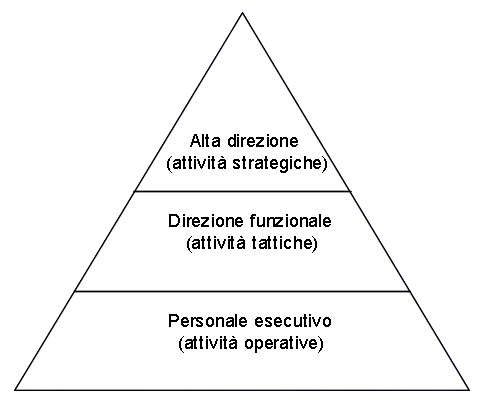
\includegraphics[scale = 0.5]{03/schemaAnthony.png}
            \caption{Schema di Anthony}
        \end{figure}\newpage
        \paragraph{profili informativi} Di seguito è riportata una tabella con i profili informativi di ciascun livello, si può notare come i livelli operativi abbiano bisogno di poche informazioni ma molto dettagliate, precise e in modo continuo, il livello direzionale tattico ha accesso ai dati con frequenza minore ma prefissata e con un livello di dettaglio minore produce quindi un volume medio di informazioni, il livello strategico ha bisogno di informazioni molto sintetizzate e con una frequenza molto bassa se non sporadica ma ha bisogno anche di informazioni esterne all'azienda.
        \begin{table}[H]
            \begin{adjustbox}{width=\textwidth}
                \begin{tabular}{|c|c|c|c|c|}
                    \hline
                    & \textbf{Frequenza} & \textbf{Dati} & \textbf{Provenienza dati} & \textbf{Volume} \\
                    \hline
                    \textbf{Livello direzionale strategico} & Sporadica & molto sintetizzati & interni ed esterni & basso \\
                    \hline
                    \textbf{Livello direzionale tattico} & Prefissata & sintetici e analitici & interni & medio \\
                    \hline
                    \textbf{Livello operativo} & Continua & analitici & interni & elevati \\
                    \hline
                \end{tabular}
            \end{adjustbox}
        \end{table}
\section{Sistemi operazionali}
    \paragraph{funzioni principali}
        \begin{itemize}
            \item Automazione di attività procedurali - In questo caso il \texttt{SI} è un supporto all'operatore
            \item Definizione di nuovi processi - come visto \hyperref[subsec:nuoviProcessi]{sottosezione 2.3.3}
            \item Aiuto nelle attività aziendali 
            \item Raccolta di dati - gli operatori inseriscono i dati nel sistema in modo continuo
            \item Guida per l'operatore - il sistema guida l'operatore nelle attività da svolgere in questo modo si riducono gli errori
        \end{itemize}
    \paragraph{Azioni sui dati}
        \begin{itemize}
            \item Accesso interattivo in inserimento, lettura, modifica - l'operatore può interagire con il sistema e modificare i dati nei limiti imposti 
            \item Trattamento di dati - il sistema tratta i dati in modo automatico e li presenta all'operatore in modo chiaro 
            \item Descrizione di eventi - il sistema descrive le transazioni e le attività svolte in modo da poterle ripetere in caso di necessità
            \item Valutazione e trattamento di informazioni utili - il sistema valuta i dati se sussistono errori e li segnala all'operatore
            \item Aggregazione per il calcolo di indicatori di stato - il sistema aggrega i dati per calcolare indicatori di stato dell'azienda
        \end{itemize}
    \paragraph{Componenti fondamentali}
        \begin{itemize}
            \item Base si dati operazionale - contiene i dati operativi dell'azienda
            \item Funzioni operative - funzioni che permettono di svolgere le attività operative
        \end{itemize}
\section{Sistemi informazionali}
    \paragraph{funzioni principali}
        \begin{itemize}
            \item Facilitazione del processo decisionale
            \item Presentazione dei dati secondo diverse aggregazioni e viste
            \item Confronto tra indicatori aziendali e indicatori esterni
        \end{itemize}
    \paragraph{Azioni sui dati}
        \begin{itemize}
            \item Accesso in lettura
            \item Aggregazione dei dati
            \item Descrizione di aree/temi
            \item Profondità temporale
            \item Multi-dimensionalità
        \end{itemize}
    \paragraph{Componenti fondamentali}
        \begin{itemize}
            \item Base dati informativa
            \item Strumenti di analisi
            \item Procedure di alimentazione (dati)
        \end{itemize}
    \chapter{Le scelte organizzative}
\thispagestyle{chapterInit}
Andiamo ora ad analizzare come il sistema informativo possa essere costruito e gestito all'interno di un'azienda. In particolare andremo ad analizzare le scelte che un'azienda può fare riguardo alla costruzione e gestione del sistema informativo, quali sono le figure professionali che si occupano di questo sulla base della dimensione dell'azienda. Andiamo inoltre ad affrontare come il sistema informativo si posiziona nell'organigramma aziendale e come l'infrastruttura tecnologica può essere organizzata e gestita.
\section{Costruzione del \texttt{SI}}
    Al momento quando si parla di adottare un nuovo \texttt{SI} si possono fare tre scelte principali:
    \begin{description}
        \item[Make] costruire il \texttt{SI} internamente
        \item[Buy] acquistare il \texttt{SI} da uno o più fornitori esterni
        \item[Outsource] far gestire ad una azienda esterna il \texttt{SI}
    \end{description}
    \subsection{Opzione \textit{make}}
    \label{sec:opzMake}
        Con l'opzione \textbf{make} ovvero di \textbf{costruzione interna} si intende la costruzione del \texttt{SI} all'interno dell'azienda da parte di un gruppo di lavoro incaricato della realizzazione, manutenzione e gestione del \texttt{SI}.\newline
        Questa opzione è raramente scelta e solitamente si limita a funzioni marginali rispetto ad un \texttt{SI} completo. Il tutto però rispecchia in pieno i modelli organizzativi e si ha un controllo totale del \texttt{SI}.
        \subsubsection{Vantaggi \& Svantaggi} 
        Questa opzione comporta dei costi fissi molto elevati usati sia per il personale che è incaricato di sviluppare e mantenere l'\texttt{SI} che per l'infrastruttura sulla quale l'\texttt{SI} è installato. Inoltre quando vi è necessità di un aggiornamento importante bisogna investire molte risorse economiche. Questa soluzione ha lo svantaggio di non confrontarsi con il mercato attuale e che dunque alcune funzionalità non sono le più efficienti o efficaci. Il primo vantaggio lo si riscontra nella situazione nella quale si dovessero verificare dei problemi, allora i tempi di risoluzione saranno molto brevi per questioni banali, ma lunghi per difficoltà più complesse. Altro vantaggio importante di questa soluzione è il mantenimento interno del ``\textit{know-how}''.
    \subsection{Opzione \textit{buy}}
        \label{sec:opzBuy}
        L'opzione \textit{buy} consiste nell'acquisto di un \texttt{SI} da parte di uno o più fornitori esterni, alla quale si aggiunge l'instaurazione di un piccolo gruppo di lavoro interno per la gestione del \texttt{SI} e per la gestione dei rapporti con i fornitori del \texttt{SI}. Questa è una scelta tipica nell'economia italiana delle \texttt{PMI}.
        \subsubsection{Vantaggi \& Svantaggi}
            Questa opzione favorisce una struttura interna umana e tecnologica di molto ridotta rispetto all'\nameref{sec:opzMake} insieme ai costi fissi. L'azienda si concentra sul proprio core business senza perdere tempo e risorse nella gestione del \texttt{SI}, questo al prezzo di una stretta dipendenza dai fornitori esterni ed una perdita \underline{parziale} del \textit{know-how} aziendale oltre alla mancata proprietà del \textit{software}. Come ulteriori vantaggi si ha la maggior flessibilità del \texttt{SI} e il confronto con il mercato attuale. Il tutto però con un modello organizzativo non su misura per l'azienda e la difficoltà nel passaggio da un fornitore all'altro.
    \subsection{Opzione \textit{outsource}}
        Con l'opzione di \textbf{outsourcing} ovvero di \textbf{esternalizzazione} si delega ad una terza parte la gestione e l'organizzazione del \texttt{SI} dopo pagamento di canone periodico.\newline
        Questa opzione al giorno d'oggi sta prendendo piede tra le \texttt{PMI} in quanto permette, seppur ad un costo variabile elevato, di avere un \texttt{SI} completo e funzionante senza dover investire in \textit{hardware} e \textit{software} e senza dover adibire personale interno alla gestione del \texttt{SI}.
        \subsubsection{\textit{Hosting}}
            Con questa opzione si affida solo la parte di \textbf{infrastruttura} tecnologica, non il \textit{software} e altri servizi che solitamente vengono gestiti in ottica \hyperref[sec:opzBuy]{\textit{buy}}. Con questa opzione si può noleggiare un server fisico o una macchina virtuale.
        \subsubsection{Body rental}
            Con questo termine intendiamo l'uso di personale specialistico di una azienda esterna per trasformare costi fissi in costi variabili.
        \subsubsection{Vantaggi \& Svantaggi}
            Nell'opzione \textit{outsource} i costi sono variabili ma abbastanza alti, inoltre in caso di necessità si può aumentare o diminuire le risorse in base alle esigenze. Si è però vincolati al fornitore della soluzione utilizzata. È presente inoltre una maggiore flessibilità rispetto all'\nameref{sec:opzMake}, come al livello dell'\nameref{sec:opzBuy}. Questa opzione però non permette di avere alcun \textit{know-how} interno e quindi non si ha la possibilità di personalizzare la soluzione in base alle proprie esigenze. Inoltre si ha una maggiore dipendenza dal fornitore del servizio. Possiamo dunque definire l'opzione \textit{outsource} come una \nameref{sec:opzBuy} con costi variabili e senza controllo su nessun aspetto del \texttt{SI}.

\section{Le figure professionali}
    \paragraph{Maturità Informatica} 
        La \textbf{maturità informatica} delle aziende è un indicatore rispetto alla diversa organizzazione e alla collocazione nell'organigramma aziendale del reparto \texttt{IT}, ovvero il reparto che si occupa della gestione del \texttt{SI}. 
    \subsection{Sviluppo del reparto}
        \subsubsection{Livello 1}
            Spesso le aziende a questo livello sono alle fasi iniziali dell'automazione.
            Il \textit{team} è composto in modo da pochi elementi, spesso non specializzati ma altamente flessibili e con competenze trasversali. Questo \textit{team} ha una struttura completamente \textbf{orizzontale} e non vi è una figura di riferimento. Può capitare che i componenti del \textit{team} siano anche responsabili di altre attività aziendali e che la parte informatica sia solo una parte del loro lavoro.
        \subsubsection{Livello 2}
            \begin{figure}[H]
                \centering 
                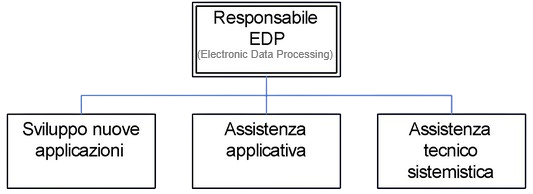
\includegraphics[width=0.5\textwidth]{04/livello2.png}
                \caption{Schema di organizzazione del reparto \texttt{IT} a livello 2}
            \end{figure}
            In questo livello si inizia ad osservare una organizzazione gerarchica dove il \textbf{responsabile \texttt{EDP}} (Electronic Data Processing) è responsabile del reparto \texttt{IT}, sotto di lui ci sono i \textbf{sistemisti} che si occupano della gestione e dell'assistenza sull'infrastruttura. Poi ci sono gli \textbf{analisti} che supportano gli utenti e analizzano i requisiti. Infine ci sono i \textbf{programmatori} che si occupano dello sviluppo del software (non presenti nell'organizzazione \hyperref[sec:opzBuy]{\textit{buy}})
        \subsubsection{Livello 3}
            \begin{figure}[H]
                \centering 
                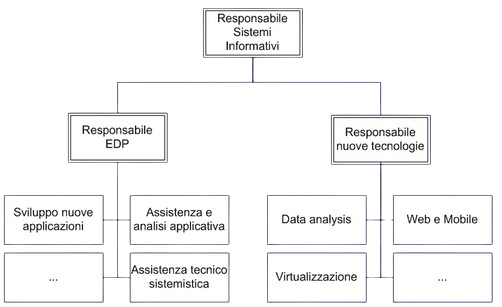
\includegraphics[width=0.5\textwidth]{04/livello3.png}
                \caption{Schema di organizzazione del reparto \texttt{IT} a livello 3}
            \end{figure}
            In questo livello è presente una vera e propria Direzione, sotto questa sono presenti i reparti di \texttt{EDP} e il reparto pero la ricerca su nuove tecnologie. Come mostrato della figura il primo si occupa di sviluppo di nuove applicazioni, assistenza e analisi e assistenza tecnico-sistemistica mentre nel secondo ci si occupa di Analisi dei dati, ricerca web e mobile e virtualizzazione della infrastruttura.
        \subsubsection{Livello 4}
            \begin{figure}[H]
                \centering 
                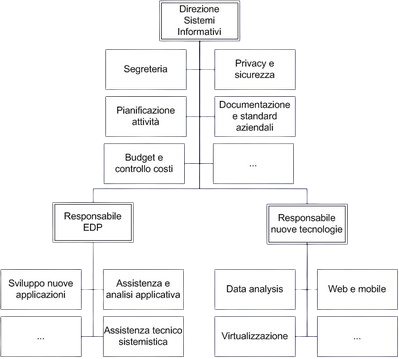
\includegraphics[width=0.5\textwidth]{04/livello4.png}
                \caption{Schema di organizzazione del reparto \texttt{IT} a livello 4}
            \end{figure}
            Livello nel quale è presente un vero e proprio \textbf{dirigente del sistema informativo} con una organizzazione gerarchica molto più complessa rispetto ai livelli precedenti. È presente una divisione \textbf{EDP} con relativo responsabile che è isolata dal reparto \textbf{nuove tecnologie} che si occupa di sviluppare nuove tecnologie e di supportare il reparto \textbf{EDP}. Inoltre sopra di questi è presente una sezione comune del sistema informativo che si occupa di coordinare i due reparti e gestire anche \textbf{privacy} e \textbf{sicurezza} o anche \textbf{pianificazione attività}. Questo livello dispone di un vero e proprio \textbf{budget} per il reparto \texttt{IT}.
    \subsection{Posizione all'interno dell'organigramma}

        Avendo definito il livello di maturità del reparto \texttt{IT} come struttura interna andiamo ora a valutare come il reparto stesso si posiziona all'interno dell'azienda, anche questo aspetto contribuisce a definire il livello di maturità dell'azienda stessa rispetto all'informatica.
        \subsubsection{Supporto amministrativo} 
            In questo caso il reparto \texttt{IT} è visto come un supporto amministrativo, questa è una visione obsoleta 
            \begin{figure}[H]
                \centering 
                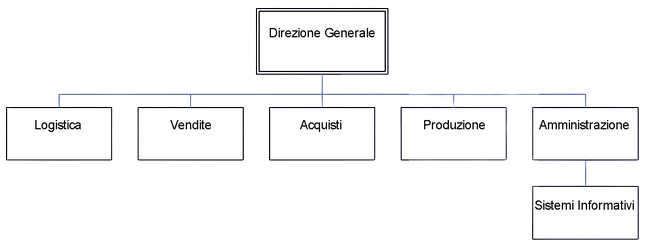
\includegraphics[width=0.5\textwidth]{04/supportoAmm.png}
                \caption{Posizione del reparto \texttt{IT} come supporto amministrativo}
            \end{figure}
        \subsubsection{Servizio ad altre direzioni generali}
            In questo caso il reparto \texttt{SI} è o al pari degli altri reparti o a supporto della direzione generale. Se il reparto \texttt{IT} è al pari degli altri reparti allora questo è a supporto di tutti i reparti dell'azienda, se invece è a supporto della \texttt{DG} allora questo si posiziona più in alto rispetto agli altri reparti.
            \begin{figure}[H]
                \centering 
                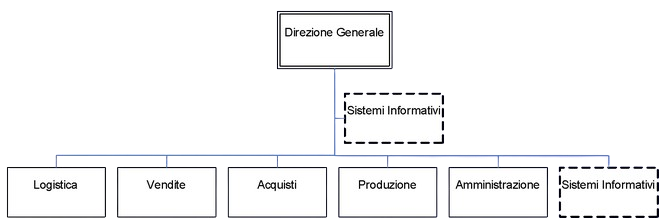
\includegraphics[width=0.5\textwidth]{04/supportoTutti.png}
                \caption{Posizione del reparto \texttt{IT} come supporto a tutte le direzioni}
            \end{figure}
        \subsubsection{Organizzazione autonoma}
            In questo caso è vero che il reparto \texttt{SI} viene messo alle dipendenze del reparto \textbf{organizzazione} ma è anche vero che in questo modello il reparto \texttt{SI} è autonomo. Il suo ruolo è quello di supportare tutte le altre direzioni e di coordinare le varie aree operative dell'azienda, solitamente questo è il modello delle grandi aziende.
            \begin{figure}[H]
                \centering 
                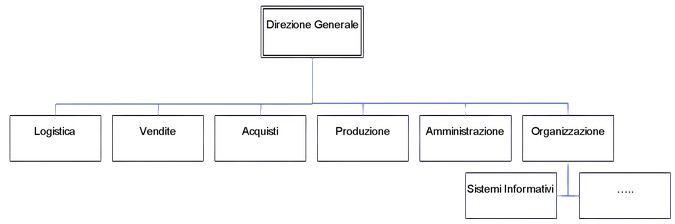
\includegraphics[width=0.5\textwidth]{04/organizzazione.png}
                \caption{Posizione del reparto \texttt{IT} come organizzazione autonoma}
            \end{figure}
\section{Infrastruttura Tecnologica}
    Negli anni l'infrastruttura tecnologica si è evoluta siamo passati da server con vari terminali connessi fino alla virtualizzazione a archiviazione in cloud, il tutto passando dall'architettura client-server. Il \texttt{SI} deve tenersi sempre aggiornato con le tecnologie in uso.
    \paragraph{Il passaggio da server locali a soluzioni cloud}
        Recentemente molte aziende stanno eseguendo il passaggio da una infrastruttura locale ad una in cloud, in questo modo sussistono meno investimenti lato \textit{hardware} e \textit{software} che ai giorni nostri invecchiano ancora prima di essere ammortizzati. Tutto il lavoro di gestione dell'infrastruttura è spostato su una azienda esterna senza che venga a mancare l'accessibilità degli strumenti informativi aziendali. In questo modo però si è \textbf{dipendenti dalla connettività} ovvero il lavoro non può essere svolto se non si è connessi a internet.
\section{Interrompibilità del servizio informatico}
    In ogni caso bisogna sempre valutare che danno può causare l'interruzione del servizio informatico. In alcuni casi l'interruzione di esso può portare al ``blocco totale'' del lavoro, questo rischio viene spesso sottovalutato dai \textit{top manger}. Come conseguenza è importante garantire la ``continuità operativa'' ovvero la riduzione o il completo annullamento che un ``blocco totale'' possa avvenire. 
    \subsubsection{Problematiche legate all'hardware}
        L'infrastruttura dei \texttt{SI} è soggetta a guasti, bisogna dunque prevenire questi andando a implementare il concetto di ``\textit{sistema ridondato}''\footnote{La ridondanza prevede che in caso di fallimento di un singolo sistema ne esista un'altro che possa sostituirsi ad esso andando a ``coprire'' il punto difettoso} (esempio per i dischi di archiviazione: \texttt{RAID}).
        \paragraph{\textit{Hot Swap}} Importante per i supporti di archiviazione è anche il concetto di \textit{Hot Swap} che consiste nella possibilità di sostituzione di questi senza dover spegnere il sistema e quindi dover interrompere l'operabilità del \texttt{SI}. 
        \paragraph{\textit{Failure tolerancy}} L'ideale infrastruttura di un \texttt{SI} dovrebbe essere \textit{fault tolerant}, ovvero non deve esistere un oggetto\footnote{server, apparato di rete, griglia elettrica, etc\dots } che in caso di fallimento comporta al fallimento di tutto il sistema, ciò per quelle parti del sistema che sono ritenute essenziali.
        \paragraph{\textit{Backup}} In ogni ambiente si rende necessaria l'implementazione di una strategia di \textit{backup}, queste copie devono essere conservate in ambienti protetti (casseforti ignifughe, locazioni remote\dots). Una teoria suggerisce che bisogni avere sempre a disposizione tre copie dei dati su tre apparati diversi: uso, \textit{backup} interno, \textit{backup} remoto.
    \subsubsection{Problematiche legate al software}
        Maggiormente le problematiche di un \texttt{SI} sono legate al \textit{software}. I problemi legati a consistono nella ``indimostrabilità'' che un qualsiasi programma  cerchi di computare un risultato senza ``ciclare'' all'infinito. D'altra parte questo genere di malfunzionamenti raramente comporta un blocco di tutto il \texttt{SI} ma più spesso interferiscono con un processo specifico o con un gruppo di attività.
    \subsubsection{Problematiche legate ad azioni dolose}
        Molto più frequenti rispetto agli altri generi di criticità sono quelle problematiche legate ad azioni intenti a ledere l'operabilità o la segretezza dei dati. Molto spesso questo genere di problematiche è causato da vulnerabilità dell'\texttt{SI} o dell'\textit{hardware}. La causa principale però rimane l'errore umano che può essere solamente mitigato.\footnote{Più informazioni sulla sicurezza informatica in ``Appunti di Introduction to Computer and Network Security'' di Luca Facchini, capitoli 1/2}
    \chapter{I sistemi operazionali}
\thispagestyle{chapterInit}
\label{ch:operazionali}
In questo capitolo verranno esposti concetti base sui ``sistemi operazionali'' parlando dunque delle finalità di questi, dell'organizzazione della informazione operativa, della potenzialità informatiche di una azienda ed infine degli accenni alla composizione di un sistema operazionale.

\section{Finalità dei sistemi operazionali}
    Le principali finalità dei \textbf{sistemi operazionali} riguardano:
    \begin{description}
        \item[Registrazione delle transazioni] Il processo di acquisizione e memorizzazione delle informazioni relative alle transazioni aziendali.
        \item[Pianificazione e controllo] La possibilità di pianificare le operazioni aziendali e controllarne l'effettiva esecuzione.
        \item[Acquisizione ed organizzazione della conoscenza] La possibilità di acquisire e organizzare la conoscenza aziendale.
        \item[Elaborazione delle situazioni aziendali] La possibilità di elaborare le informazioni aziendali per ottenere una visione complessiva della situazione aziendale.
    \end{description}
    Per raggiungere questa finalità il sistema operazionale si compone di due sottosistemi principali:
    \begin{description}
        \item[Base di dati operazionale] Contiene le informazioni operative in forma organizzata.
        \item[Funzioni operative] Sono le funzioni che permettono di acquisire, memorizzare, elaborare e trasmettere le informazioni.
    \end{description}
    \subsection{Transazioni - Definizione e registrazione}
        \subsubsection{Cos'è una transazione}
            \paragraph{Definzione} Per definizione una \textbf{transazione} è una operazione detta \textbf{atomica} (ovvero indivisibile) che si manifesta in un certo e conosciuto momento ed è una informazione che l'azienda è interessata a registrare.
            \paragraph{Esempi} Alcuni esempi di transazioni sono: gli ordini tra cliente e fornitori, prelievi da magazzino, spedizioni, pagamenti, ecc\dots
        \subsubsection{Registrazione delle transazioni}
            Le transazioni da dover registrare, possono essere sostanzialmente di due tipi:
            \begin{description}
                \item[Semplici] Si deve registrare nel sistema solo un singolo dato.
                    \subitem Esempio di registrazione di transazione semplice è la registrazione di una movimentazione del magazzino
                \item[Complesse] Si devono registrare più operazioni elementari connesse in senso logico e spesso corelate a documenti fisici, quali ad esempio una spedizione che è correlata ad una \textit{bolla di spedizione}.
                    \subitem Esempio di registrazione di transazione complessa è la registrazione di una spedizione dove sono coinvolte più operazioni elementari quali la raccolta degli attributi (destinatario, prodotti, data e ora\dots) ed genera una bolla di spedizione.
            \end{description}
            Inoltre una transazione può generarle delle altre e quindi si parla di \textbf{transazioni a cascata}.
            \paragraph{Volume dei dati} Ogni transazione produce un volume di dati dipendentemente dalla natura dell'attività e dell'organizzazione aziendale.
    \subsection{Pianificazione e controllo delle operazioni}
        Alcuni processi aziendali sono dipendenti da altri, si rende quindi necessario usare i dati dei processi ``a monte'' per pianificare e controllare i processi ``a valle''. Tramite l'uso di \texttt{SI} è possibile adottare modelli più complessi di pianificazione e monitorare continuativamente l'andamento dello stato dei processi aziendali. 
        \paragraph{Perché pianificare e controllare} Pianificare e controllare i processi aziendali ha diversi vantaggi per l'azienda, sia per il passato che per il presente fino ad avere anche una utilità per i processi futuri. Questi vantaggi sono raggiunti tramite: La possibilità di elaborare piani e strategie di produzione, registrare e monitorare l'avanzamento delle operazioni ed infine la possibilità di misurare se e quanto i piani sono stati rispettati rispetto agli obiettivi prefissati.
            \subparagraph{Come pianificare e controllare} Il \texttt{SI} deve essere dotato di funzioni molto articolate e specifiche per l'azienda alla quale si riferisce, ad esempio quando parliamo di ``Elaborazione di piani'' il \texttt{SI} di riferimento deve essere in grado di: ottimizzare le risorse disponibili, sincronizzare le operazioni ed essere coerente con lo stato degli indicatori aziendali.
    \subsection{Organizzazione della conoscenza aziendale}
        La conoscenza aziendale (\textit{Knowledge Base} - \texttt{KB}) è l'insieme delle informazioni a supporto dell'attività di produzione aziendale, come ad esempio le informazioni sui prodotti, sui processi, sui clienti, sui fornitori, ecc\dots Queste informazioni sono essenziali per la gestione aziendale e per la pianificazione delle attività future, avere dunque all'interno del \texttt{SI} operazionale la loro versione più aggiornata sempre a disposizione è fondamentale per l'azienda.\newline
        Queste informazioni devono essere strutturate, ovvero riconducibili ad un insieme di caratteristiche predefinite, e devono essere corelate, ovvero devono essere collegate ad articoli, clienti, fornitori, ecc\dots
    \subsection{Elaborazione delle situazioni aziendali}
        Il \texttt{SI} è un sistema dinamico che serve per modellare la realtà aziendale e per fornire informazioni utili per la gestione aziendale. La conoscenza dello stato corrente, oltre che di quello passato, è fondamentale per la gestione aziendale, questa conoscenza permette di pilotare l'azienda grazie a determinati eventi. Alcuni indicatori di stato sono ad esempio: le giacenze di magazzino, i tempi di consegna, i tempi di produzione, ecc\dots\newline
        Gli indicatori dunque non rappresentano una situazione statica, ma una situazione dinamica che cambia nel tempo. Questi indicatori sono utili per la gestione aziendale e per la pianificazione delle attività future. Tutti gli indicatori di stato sono calcolati a partire dai dati inseriti, modificati e cancellati dalle transazioni aziendali e sono utili per la gestione aziendale.
\section{Informazione Operativa}
    L'informazione operativa è costituita principalmente da archivi nei quali sono presenti relazioni che coinvolgono diverse entità, questi archivi solitamente li classifichiamo in:
    \begin{description}
        \item[Movimenti] Contengono le informazioni relative alle transazioni semplici, relative ad un singolo oggetto.
        \item[Documenti] Contengono le informazioni su transazioni complesse che riguardano una lisa di oggetti (classica tabella) dove in testa troviamo anche una serie di informazioni comune a tutte le righe.
        \item[Informazioni di stato] Ovvero un insieme di indicatori di stato che permettono di avere una visione complessiva della situazione aziendale. Questi possono essere \textit{de-materializzati} e quindi calcolati al momento della richiesta o \textit{materializzati} e quindi calcolati e memorizzati in un archivio.
        \item[Informazioni Anagrafiche] Contengono le informazioni relative alle entità che partecipano alle transazioni, questi non si limitano a contenere solo dati di anagrafica di persone fisiche, ma anche di oggetti, di entità giuridiche, ecc\dots
    \end{description}
    \subsection{Qualità dei dati}
        Per qualità dei dati si fà riferimento allo standard \texttt{ISO 8402-1995}:
        \begin{quote}[\texttt{ISO 8402-1995}]{\textit{International Organization for Standardization}}
            Il possesso della totalità delle caratteristiche che portano al soddisfacimento delle esigenze espresse o implicite, dell'utente.
        \end{quote}
        \paragraph{La qualità dei dati}
            Per stabilire un indice di qualità dei dati si possono utilizzare diversi parametri quali:
            \begin{itemize}
                \item Tanto più elevata quanto più il sistema fornisce rappresentazioni degli eventi vicine alla percezione diretta della realtà
                \item La dipendenza dalla struttura del \texttt{SI} è minore quanto più i dati sono indipendenti dalla struttura del sistema
                \item La qualità è diminuita da sottosistemi non integrati e da dati ridondanti
            \end{itemize}
            In sostanza un dato per essere di qualità non deve essere ridondante, deve essere coerente con la realtà e deve essere indipendente dalla struttura del sistema.
        \paragraph{Impatto della qualità dei dati}
            Se all'interno del proprio \texttt{SI} si ha una bassa qualità dei dati, allora si avrà un forte impatto economico/organizzativo tra cui: la difficoltà nell'introduzione di innovazioni tecnologiche (adozione di una nuova tecnologia) e di processo (modificare un processo produttivo), la difficoltà nell'avvio di processi del tipo \textit{data warehousing}, inoltre dal lato umano avere una bassa qualità dei dati può portare a una scarsa soddisfazione degli utenti finali del \texttt{SI} (ovvero quelle persone che utilizzano il \texttt{SI} per svolgere il proprio lavoro).
    \subsection{Caratteristiche strutturali}
        L'informazione operativa è l'informazione che serve per svolgere le attività operative dell'azienda, questa informazione è costituita da dati che vengono acquisiti, memorizzati, elaborati e trasferiti all'interno dell'azienda. Questi dati sono utili per la gestione aziendale e per la pianificazione delle attività future. L'informazione operativa è caratterizzata da:
        \begin{description}
            \item[Aggregazione] I dati sono aggregati in base alle esigenze dell'utente, possono essere:
                \subitem \textbf{Analitici} Se si vuole avere una visione dettagliata di un singolo evento.
                \subitem \textbf{Analitici} Se si vuole avere una visione complessiva di un insieme di eventi, ottenuto aggregando i dati.
            \item[Tempificazione] I dati possono essere temporizzati in base alle esigenze dell'utente, possono essere:
                \subitem \textbf{Puntuale} Se si vuole avere una visione istantanea della situazione aziendale.
                \subitem \textbf{Cumulata} Se si vuole avere una visione della situazione aziendale in un certo periodo di tempo.
            \item[Dimensionalità] Intendiamo come dimensionalità il numero minimo di parametri necessari per estrarre una specifica informazione.
        \end{description}
        Esempio delle caratteristiche dell'informazione operativa:
        \begin{table}[H]
            \centering
            \begin{tabular}{|c|c|c|c|}
                \hline
                & \textbf{Aggregazione} & \textbf{Tempificazione} & \textbf{Dimensionalità} \\
                \hline
                \textbf{Anagrafe} & Analitica & Puntuale & unitaria \\
                \hline
                \textbf{Movimenti \& Documenti} & Analitica & Puntuale & Contenuta \\
                \hline
                \textbf{Informazioni di stato} & Analitica o aggregata & Puntuale o cumulata & Contenuta \\
                \hline
            \end{tabular}
        \end{table}
    \subsection{Caratteristiche funzionali}
        I dati operativi oltre ad essere strutturati in maniera particolare, devono anche avere delle caratteristiche funzionali che permettano di svolgere le attività operative dell'azienda. Queste caratteristiche sono:
        \begin{description}
            \item[Completezza] Estensione con cui i dati vengono registrati
            \item[Corretteza] Quanto quel dato si avvicina alla realtà
            \item[Precisione] Quanto quel dato è vicino alla realtà
            \item[Omogeneità] Se tra tutti i dati della stessa natura sono rappresentati con una stessa struttura
            \item[Fruibilità] Facilità con cui i dati possono essere reperiti, acquisiti e compresi dall'utente in relazione alle sue esigenze
        \end{description}

\footnote{
    La sezione 4.3 del libro ``Rappresentazione della realtà'' è stata omessa in quanto trattata marginalmente a lezione ed approfondita al corso di \textit{Basi di Dati}.
}
\section{Potenzialità informatica}
    \begin{definition}[Potenzialità informatica]
        La \textbf{potenzialità informatica} è costituita principalmente da due indicatori:
        \begin{description}
            \item[Intensità informativa] Misura la quantità di informazioni della quale l'azienda necessita, sia che queste vengano da fonti interne o esterne.
            \item[Attrattiva informatica] Ovvero la propensione, sulla base dei processi aziendali, dell'azienda ad utilizzare un \texttt{SI} per la gestione delle informazioni.
        \end{description}
    \end{definition}
    Inoltre la propensione del management verso l'investimento sulla infrastruttura informatica è un indicatore di potenzialità informatica. 
    \subsection{Intensità informativa}
        \begin{definition}[Intensità informatica]
            L'intensità informativa è costituita da un insieme di fattori che concorrono a determinare la quantità di informazioni di cui l'azienda necessita. 
        \end{definition}
        Questi fattori sono:
        \begin{itemize}
            \item La complessità dell'attività aziendale: oltre alla dimensione dell'azienda và presa in considerazione l'area geografica l'eventuale appartenenza ad un ``gruppo'', il livello di diversificazione dei prodotti, dei mercati e delle tecnologie. Tutti questi fattori influenzano la quantità di informazioni necessarie.
            \item L'intensità informativa
        \end{itemize}
    \begin{definition}[Intensità informativa]
        L'intensità informativa è costituita dal prodotto dell'intensità informativa di prodotto e dell'intensità informativa di processo.
    \end{definition}
    \begin{definition}[Intensità informativa di prodotto]
        L'intensità informativa di prodotto è la quantità di informazioni necessarie per la progettazione, la produzione e la commercializzazione di un prodotto.
    \end{definition}
    \begin{definition}[Intensità informativa di processo]
        L'intensità informativa di processo è la quantità di informazioni necessarie per l'avanzamento dei processi aziendali. Viene presa in considerazione anche la mole di dati che emergono dal processo e la complessità delle operazioni elementari previste dal processo.
    \end{definition}
    \subsection{Attrattiva Informatica}
        L'intensità informativa non è sufficiente a determinare se l'adozione di un \texttt{SI} possa essere vantaggiosa per l'azienda, infatti è necessario anche valutare l'attrattiva informatica.
        \begin{definition}[Attrattiva informatica]
            L'attrattiva informatica è un indicatore che misura la propensione dell'azienda ad utilizzare un \texttt{SI} per la gestione delle informazioni. Questo indicatore è costituito dall'insieme dell'attrattiva informatica dei processi aziendali.
        \end{definition}
        \begin{definition}[Attrattiva informatica di processo]
            L'attrattiva informatica di processo è costituita dai seguenti fattori:
            \begin{description}
                \item[Proceduralità] Grado di formalizzazione dei processi aziendali. Più un processo è formalizzato, più è attrattivo.
                \item[Complessità] Grado di difficoltà delle azioni elementari previste dal processo. Meno un processo è complesso e più è attrattivo.
                \item[Ripetitività] Frequenza con cui un processo viene ripetuto. Più un processo è ripetuto, più è attrattivo.
                \item[Volume] Quantità di dati e informazioni elaborate dal processo. Alti volumi di dati rendono un processo attrattivo         
            \end{description}
        \end{definition}
\section[Composizione dei \texttt{SI} Operazionali]{Composizione dei sistemi informativi operazionali}
    I \texttt{SI} operazionali sono composti da diversi sotto-sistemi che si occupano di diverse funzioni. Al momento non esiste una classificazione standard dei sotto-sistemi in quanto varia in base all'azienda e al settore di appartenenza. I criteri principali usati per la distinzione tra diversi sotto-sistemi sono: la funzione svolta, il processo aziendale coinvolto, l'architettura tecnologica, ecc\dots
    \subsubsection{Portafoglio Applicativo}
        Definiamo come \textbf{portafoglio applicativo} l'insieme delle applicazioni software che costituiscono il \texttt{SI} operativo, possono essere individuate due aree principali, ovvero il \textbf{portafoglio operativo} e il \textbf{portafoglio istituzionale}.
        \paragraph{Portafoglio Operativo} È costituito da applicazioni informatiche che trattano di processi legati al \textit{core-business} dell'azienda. Questo genere di portafoglio è caratterizzato da una elevata specializzazione ad un settore specifico oltre ad una elevata variabilità tra aziende dello stesso settore di appartenenza. Inoltre questo portafoglio è caratterizzato da una forte verticalizzazione e da una elevata specializzazione delle funzioni implementate.
        \paragraph{Portafoglio istituzionale} È costituito da applicazioni informatiche che trattano di processi a sostegno delle principali attività aziendali. Questo genere di portafoglio è caratterizzato da una elevata attrattiva informatica e da una alta proceduralita (e ripetitività) dei processi. Inoltre questo genere di portafoglio è caratterizzato da una elevata omogeneità tra aziende anche di settori diversi e la poca variabilità tra servizi e prodotti offerti.
    \subsubsection{Sistema gestionale classico}
        Nel modello del sistema gestionale classico solitamente sono presenti delle isole informatiche autonome e molto specializzate, questo genere di sviluppo è causato principalmente da uno sviluppo incrementale (ovvero lo sviluppo viene eseguito a compartimenti ``stagni'' uno per volta), da una rigidità delle organizzazioni aziendali, dalla specializzazione dei produttori di software ecc\dots
        \paragraph{Problematiche} Questo genere di sviluppo porta a diverse problematiche quando si discute sulla gestione dei dati, in questo sistema infatti i dati sono ridondanti, disomogenei e spesso incoerenti. Ad aggiungersi a ciò questo genere di gestionale rende difficile avere una visione complessiva dell'azienda.
        \begin{figure}[H]
            \centering
            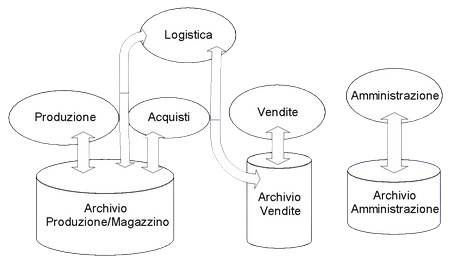
\includegraphics[width=0.5\textwidth]{05/gestionaleClassico.png}
            \caption{Schema dei settori di un sistema gestionale classico}
        \end{figure}
    \subsubsection{Sistema \texttt{ERP} - \textit{Enterprise Resource Planning}}
        Un sistema \texttt{ERP} è un sistema informativo aziendale integrato, ovvero un sistema che permette di gestire in maniera integrata e coordinata tutte le informazioni aziendali. Questo genere di sistema, grazie ad una basi di dati unica ed a processi integranti e cooperanti, punta a trattare i dati in modo ottimale e ottimizzato, oltre a gestire il controllo dei processi aziendali.
        \paragraph{Vantaggi} Questo genere di sistema così implementato è molto flessibile ed in grado di assecondare l'azienda in ogni sua esigenza, inoltre permette di avere una visione complessiva dell'azienda e di avere una gestione ottimale dei processi aziendali. Inoltre questo si adatta molto rispetto all'organizzazione aziendale e all'architettura tecnologica.
        \begin{figure}[H]
            \centering
            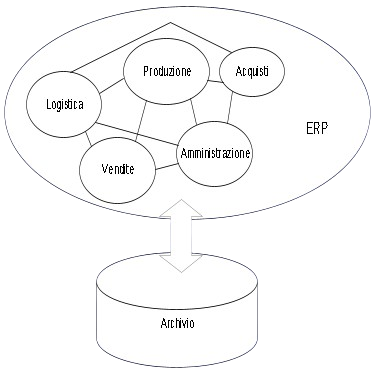
\includegraphics[width=0.33\textwidth]{05/gestionaleERP.png}
            \caption{Schema dei settori di un sistema gestionale \texttt{ERP}}
        \end{figure}
    \subsubsection{Ambiti applicativi}
        La presenza di moduli indipendenti presente negli \texttt{ERP} rendono questi sistemi molto flessibile anche a tipologie diverse di aziende, infatti un \texttt{ERP} può essere utilizzato in diversi ambiti applicativi, anche molto diversi tra loro. Tra questi ambiti troviamo: Servizi Finanziari, Produzione, Distribuzione, Commercio, Servizi, ecc\dots
        \paragraph{Flussi di base} I flussi di base di un \texttt{ERP} sono:
        \begin{description}
            \item[Amministrativo] Flusso di prima applicazione che riguarda la gestione amministrativa dell'azienda.
            \item[Logistico] Flusso che riguarda la gestione dei processi logistici dell'azienda.
            \item[Attivo (vendite)] Flusso che riguarda la gestione delle vendite dell'azienda.
            \item[Passivo (acquisti)] Flusso che riguarda la gestione degli acquisti dell'azienda.
            \item[Produttivo] Uno trai flussi più complessi, riguarda la gestione della produzione dell'azienda, questo può variare anche di molto da azienda ad azienda. 
        \end{description}
    \subsubsection{Sistemi operazionali complementari}
        I sistemi operazionali complementari sono sistemi che vengono aggiunti al sistema operativo principale per coprire delle funzioni che non sono presenti nel sistema operativo principale. Questi sistemi sono caratterizzati da una forte specializzazione e da una forte integrazione con il sistema operativo principale.
        \paragraph{Esempi di sistemi operazionali complementari} Alcuni esempi di sistemi operazionali complementari sono: i sistemi di supporto alle decisioni, i sistemi di gestione della qualità, i sistemi di gestione ambientale, le estensioni dell'\texttt{ERP} ecc\dots
    \chapter{I sistemi Informazionali}
\thispagestyle{chapterInit}
\section{In generale}
    \subsection{Gli Obbiettivi}
        Gli obbiettivi principali di un sistema informazionale sono diversi, tra i quali troviamo:
        \begin{enumerate}
            \item Il sistema informazionale come strumento a supporto delle decisioni
            \item Interrogazione dei dati
            \item Base di dati
            \item Strumenti di analisi dei dati
        \end{enumerate}
        \paragraph{Sistema informazionale come supporto alle decisioni} Il sistema informazionale deve essere uno strumento al supporto delle decisioni tramite l'elaborazione di dati, prima dei sistemi informazionali questi venivano forniti tramite \textit{report} i quali però presentano \textit{bias} basati sulla persona che lo prepara (come dati omessi o punti di enfasi), inoltre risultano statici e difficili nella loro creazione. Altri strumenti superati grazie ai sistemi informazionali sono i fogli di calcolo, i quali sono soggetti a errori, è difficile collaborare e sono difficili da mantenere in quanto se si vuole modificare una formula bisogna modificarla in tutti i fogli di calcolo distribuiti.
        \paragraph{Sistema informazionale come strumento di interrogazione dei dati} Le interrogazioni si suddividono principalmente in: interrogazioni puntuali e interrogazioni complesse. Esempio di interrogazione puntuale è la ricerca della modalità di pagamento di un dato cliente, mentre un esempio di interrogazione complessa è l'analisi dell'aumento del margine operativo per una serie di prodotti rispetto all'anno precedente.
        \paragraph{Sistema informazionale come strumento di accesso alla base di dati} Il sistema informazionale deve offrire agli utenti finali un modello intuitivo ed efficiente per l'analisi, inoltre deve garantire la possibilità di integrare da fonti diverse i dati ed offrire processi di aggiornamento di questi.
        \paragraph{Sistema informazionale come strumento di analisi dei dati} In questo caso il sistema informazionale deve offrire strumenti di analisi dei dati, come \textit{reporting} di dati, oppure offre dei sistemi per l'analisi interattiva da una ipotesi iniziale oppure offre sistemi di \textit{Data Mining}
    \subsection{Terminologia}
        \paragraph{\textit{Data Warehouse}} Il \textit{Data Warehouse} è quell'insieme di tecniche per definire, costruire e mantenere un \textit{Data Base} che sia orientato all'analisi dei dati. Questo \textit{Data Base} deve essere molto strutturato e i dati organizzati in maniera efficiente per permettere l'analisi dei dati.
        \paragraph{\textit{Decision Support System} - \texttt{DSS}} Il \texttt{DSS} è una parte del sistema informazionale che integrato nel processo decisionale dell'azienda, permette di visualizzare ed estrarre le informazioni da basi di dati ben organizzate
        \paragraph{\textit{Data mining}} Il \textit{Data Mining} è una tecnica che permette di estrarre informazioni utili da un grande insieme di dati, questa tecnica è utilizzata per scoprire relazioni tra i dati e per fare previsioni.
        \paragraph{\textit{Buisness Intelligence}} Ovvero tutte le attività di estrazione di informazioni dai dati di \textit{business} generati dai processi operativi aziendali.
        \paragraph{\textit{Knowledge Management}} Ovvero l'insieme della conoscenze che ogni individuo possiede i quali dovrebbero essere distribuiti in maniera efficiente all'interno del sistema informazionale. Spesso questa conoscenza è derivata da esperienze passate, da informazioni acquisite e da competenze acquisite, alcune volte questa conoscenza è difficile da trasferire ed è difficile da codificare.
        \paragraph{\textit{Big Data}}
    \subsection{Le caratteristiche}
        \paragraph{Finalità} Il sistema informazionale deve essere in grado di fornire un substrato informativo per la conoscenza dell'azienda, inoltre deve essere in grado di descrivere il passato ed aiutare ad identificare i problemi e le loro cause. Inoltre deve poter suggerire i cambiamenti da apportare e fornire anticipazioni sui scenari futuri.
        \paragraph{Struttura} I dati devono essere articolati intorno ai soggetti di cui si vuol conoscere l'apporto alla vita aziendale
        \paragraph{Utenza} I principali utenti del sistema informazionale sono i manager e i decisori che devono avere una visione e conoscenza ampia dell'azienda
        \paragraph{Storicità} Il sistema deve mantenere e fornire uno storico dei dati con un arco temporale adeguato e molto più esteso rispetto a quello dei sistemi operazionale, inoltre deve fornire l'evoluzione storia dei soggetti di interesse.
        \paragraph{Dettaglio} I dati sono quasi esclusivamente in forma aggregata e devono essere disponibili a diversi livelli di aggregazione.
        \paragraph{Accesso} L'accesso ai dati è principalmente solo in lettura, eventuali aggiornamenti sono solo periodici e in momenti nei quali l'attività aziendale è ferma.
\section{Modello multidimensionale}
    \subsection{Introduzione}
        Il modello multidimensionale è un modello di rappresentazione dei dati che permette di rappresentare i dati in maniera più intuitiva rispetto al modello relazionale. In questo modello il processo di analisi viene posto al centro del sistema e non più il processo di inserimento dei dati (i quali vengono inseriti non in maniera diretta ma vengono estratti da un \texttt{SI} Operazionale\footnote{Si rimanda al capitolo: \ref{ch:operazionali} \nameref{ch:operazionali} per ulteriori informazioni sui sistemi operazionali}).
        In questo modello lo spazio delle informazioni viene rappresentato come insieme di matrici multidimensionali, dove ogni matrice rappresenta un tipo di evento (quale ad esempio l'immatricolazioni degli studenti), ogni elemento della matrice rappresenta un singolo evento (la singola immatricolazione) e ogni coordinata della matrice rappresenta una dimensione dell'evento (come ad esempio il corso di laurea, l'anno di immatricolazione, ecc\dots).
\end{document}